%%%%%%%%%%%%%%%%%%%%%%%%%%%%%%%%%%%%%%%%%
% University Assignment Title Page 
% LaTeX Template
% Version 1.0 (27/12/12)
%
% This template has been downloaded from:
% http://www.LaTeXTemplates.com
%
% Original author:
% WikiBooks (http://en.wikibooks.org/wiki/LaTeX/Title_Creation)
%
% License:
% CC BY-NC-SA 3.0 (http://creativecommons.org/licenses/by-nc-sa/3.0/)
% 
% Instructions for using this template:
% This title page is capable of being compiled as is. This is not useful for 
% including it in another document. To do this, you have two options: 
%
% 1) Copy/paste everything between \begin{document} and \end{document} 
% starting at \begin{titlepage} and paste this into another LaTeX file where you 
% want your title page.
% OR
% 2) Remove everything outside the \begin{titlepage} and \end{titlepage} and 
% move this file to the same directory as the LaTeX file you wish to add it to. 
% Then add \input{./title_page_1.tex} to your LaTeX file where you want your
% title page.
%
%%%%%%%%%%%%%%%%%%%%%%%%%%%%%%%%%%%%%%%%%
%\title{Title page with logo}
%----------------------------------------------------------------------------------------
%	PACKAGES AND OTHER DOCUMENT CONFIGURATIONS
%----------------------------------------------------------------------------------------

\documentclass[12pt]{article}
\usepackage[italian]{babel}
\usepackage[utf8x]{inputenc}
\usepackage{amsmath}
\usepackage{graphicx}
\usepackage[colorinlistoftodos]{todonotes}
\usepackage{float}

\begin{document}

\begin{titlepage}

\newcommand{\HRule}{\rule{\linewidth}{0.5mm}} % Defines a new command for the horizontal lines, change thickness here

\center % Center everything on the page
 
%----------------------------------------------------------------------------------------
%	HEADING SECTIONS
%----------------------------------------------------------------------------------------

\textsc{\LARGE Università degli studi di Milano-Bicocca}\\[1cm] % Name of your university/college
\textsc{\Large Advanced Machine Learning }\\[0.3cm] % Major heading such as course name
\textsc{\large Progetto Finale}\\[0.1cm] % Minor heading such as course title

%----------------------------------------------------------------------------------------
%	TITLE SECTION
%----------------------------------------------------------------------------------------

\HRule \\[0.4cm]
{ \huge \bfseries Overfitting}\\[0.4cm] % Title of your document
\HRule \\[1.5cm]
 
%----------------------------------------------------------------------------------------
%	AUTHOR SECTION
%----------------------------------------------------------------------------------------

\large
\emph{Autori:}\\
Lorenzo Mammana - 807391- l.mammana@campus.unimib.it \\   % Your name
Eric Nisoli - 807147- e.nisoli1@campus.unimib.it   \\[1cm] % Your name

% If you don't want a supervisor, uncomment the two lines below and remove the section above
%\Large \emph{Author:}\\
%John \textsc{Smith}\\[3cm] % Your name

%----------------------------------------------------------------------------------------
%	DATE SECTION
%----------------------------------------------------------------------------------------

{\large \today}\\[2cm] % Date, change the \today to a set date if you want to be precise

%----------------------------------------------------------------------------------------
%	LOGO SECTION
%----------------------------------------------------------------------------------------


\includegraphics{logo.png}\\[1cm] % Include a department/university logo - this will require the graphicx package
 
%----------------------------------------------------------------------------------------

\vfill % Fill the rest of the page with whitespace

\end{titlepage}


\begin{abstract}
The ABSTRACT is not a part of the body of the report itself. Rather, the abstract is a brief summary of the report contents that is often separately circulated so potential readers can decide whether to read the report. The abstract should very concisely summarize the whole report: why it was written, what was discovered or developed, and what is claimed to be the significance of the effort. The abstract does not include figures or tables, and only the most significant numerical values or results should be given.
\end{abstract}

\section{Introduzione}
L'obiettivo del progetto è quello di costruire un modello di machine learning per la classificazione di immagini in grado di operare bene su un dataset di piccole dimensioni comprendente un alto numero di classi simili tra di loro.
Come è facilmente intuibile, il problema principale di operare su un dataset di questo tipo è l'overfitting del modello sui dati di training con conseguente fallimento del modello su dati nuovi. Per risolvere questo problema ci siamo concentrati sulla ricerca di modelli, iperparametri e tecniche di generalizzazione che permettessero al modello di essere in grado di operare su un dataset di test molto più ampio di quello utilizzato per l'addestramento.
Il modello utilizzato per questo tipo di analisi è una rete neurale convoluzionale; questo tipo di modello si è dimostrato negli ultimi anni il migliore nel classificare immagini in moltissimi campi di applicazione.

The introduction should provide a clear statement of the problem posed by the project, and why the problem is of interest. It should reflect the scenario, if available. If needed, the introduction also needs to present background information so that the reader can understand the significance of the problem. A brief summary of the hypotheses and the approach your group used to solve the problem should be given, possibly also including a concise introduction to theory or concepts used later to analyze and to discuss the results.


\section{Dataset}
Il dataset utilizzato è il \textit{102 Category Flower Dataset} creato dai ricercatori del \textit{Visual Geometry Group} di \textit{Oxford}. Il dataset è composto da 8189 immagini RGB di dimensione variabile, ogni immagine contiene uno o più fiori su sfondo neutro ed è etichettata con una singola categoria estratta da un insieme di centodue possibili. 
E' stata mantenuta la suddivisione del dataset definita nella pubblicazione originale, in particolare si hanno:
\begin{itemize}
\item 1020 immagini nel training set
\item 1020 immagini nel validation set
\item 6149 immagini nel test set
\end{itemize}
Ogni categoria è rappresentata da 10 immagini nel training set e nel validation set, mentre la proporzione di immagini per ogni categoria varia nel test set.
La difficoltà di operare su un dataset di questo tipo è evidente, il numero di immagini è limitato mentre il test set è ampio.
Mettere immagini dataset

In this section the available data sets must be presented. The term dataset refers to any type of information source, for example web services for geolocation fall into this category. 
In addition, all necessary data manipulation processes, such as cleaning and enrichment with external sources, must be presented and discussed.

\section{The Methodological Approach}
Per classificare le immagini nelle classi corrette si è deciso di utilizzare una rete neurale convoluzionale (CNN). Come è noto addestrare questo tipo di modello da zero richiede un numero di immagini dell'ordine di milioni di elementi, non avendo a disposizione così tante immagini è necessario eseguire la tecnica nota come \textit{finetuning} in cui la CNN viene inizializzata con pesi calcolati su un dataset di milioni di immagini e modificati in accordo con i propri dati disponibili.
In particolare si è deciso di utilizzare reti preaddestrate sul dataset Imagenet contenente più di 10 milioni di immagini di cui più di trecentomila rappresentanti fiori.
\subsection{Esperimento baseline}
Considerando il fatto che il numero di immagini di training è limitato è stato inizialmente deciso di definire un modello baseline non particolarmente complesso. Il modello scelto è una \textit{Resnet-18} preaddestrata su \textit{Imagenet}. Inizialmente si è provato ad utilizzare la rete come estrattore di features per valutare quanto il preaddestramento influisca sulla classificazione finale. 
Le features estratte vengono classificate utilizzando un semplice percettrone multistrato:
\begin{table}[H]
\centering
\begin{tabular}{lll}
\hline
Layer (type)     & Output Shape & Param \# \\ \hline
dense\_1 (Dense) & (None, 256)  & 6422784  \\ \hline
dense\_2 (Dense) & (None, 128)  & 32896    \\ \hline
dense\_3 (Dense) & (None, 102)  & 13158    \\ \hline
\end{tabular}
\label{t_mlp}
\caption{Architettura del percettrone}
\end{table}
\subsubsection{Preprocessing e Data augmentation}
Prima di procedere con l'estrazione delle features le immagini vengono normalizzate per avere media nulla e varianza unitaria utilizzando la formula:
\begin{equation}
x' = \frac{x - \overline{x}}{\sigma}
\end{equation}
Dove $ \overline{x} $ e $ \sigma $ rappresentano rispettivamente la media e la varianza calcolate su \textit{Imagenet}.
Questo permette di passare alla rete delle immagini più simili a quelle su cui è stata addestrata ottenendo potenzialmente delle features più discriminative.
\subsubsection{Scelta degli iperparametri}
Per addestrare il percettrone sulle features estratte si è deciso di utilizzare il semplice mini-batch stochastic gradient descent (SGD), con dimensione del batch pari a 64 e momentum pari a 0.9.
Il learning rate viene calcolato in accordo con l'algoritmo descritto in \textit{Cyclical Learning Rates for Training Neural Networks}.
Questo algoritmo prevede che il learning rate oscilli avanti ed indietro in un range prefissato di valori, questo ha un duplice scopo:
\begin{itemize}
\item Uscire da punti di sella o da minimi locali che potrebbero bloccare la corretta convergenza dell'ottimizzatore.
\item Ridurre il bias introdotto dalla scelta iniziale di un learning rate scorretto.
\end{itemize}
Per calcolare il range su cui far variare il learning rate viene utilizzata una tecnica automatizzata così funzionante:
\begin{enumerate}
\item Si definiscono un estremo inferiore piccolo ed un estremo superiore grande su cui far variare il learning rate, ad esempio [1e-10, 1e-1].
\item Si addestra la rete per un numero ridotto di epoche partendo dall'estremo inferiore ed incrementando esponenzialmente il learning rate ad ogni batch.
\item Il training continua fino a quando il learning rate non raggiunge l'estremo superiore
\item Viene plottato un grafico che mostra quando il learning rate è troppo basso o troppo alto.
\end{enumerate} 
L'algoritmo sul percettrone multistrato produce il seguente grafico:
\begin{figure}[ht]
\centering
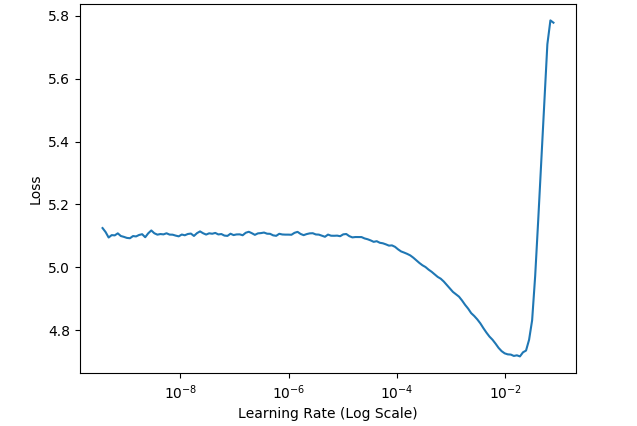
\includegraphics[width=1.0\textwidth]{images/baseline/lrfind_plot.png} 
\label{i_baseline_finder}
\caption{Output dell'algoritmo di ricerca del learning rate}
\end{figure}
\newpage
Dal grafico si vede come la rete cominci ad apprendere circa a partire da 1e-5 e diverga una volta superato 1e-2, questi due valori verranno quindi utilizzati come estremi per l'algoritmo di cyclical learning rate.
Questo algoritmo ha due ulteriori iperparametri, il primo è definito \textit{Step size} ed indica il numero di iterazioni richiesto per passare dal minimo learning rate al massimo, il secondo è il metodo con cui viene modificato il learning rate.
La rete viene addestrata per 50 epoche con diverse coppie di iperparametri; i risultati sono riportati in tabella.
\begin{table}[H]
\centering
\begin{tabular}{|l|l|l|}
\hline
Metodo       & Step size & Test accuracy \\ \hline
Triangular   & 2         & 0.550         \\ \hline
Triangular   & 4         & 0.550         \\ \hline
Triangular   & 6         & 0.558         \\ \hline
Triangular   & 8         & 0.547         \\ \hline
Triangular2  & 2         & 0.510         \\ \hline
Triangular2  & 4         & 0.527         \\ \hline
Triangular2  & 6         & 0.550         \\ \hline
Triangular2  & 8         & 0.533         \\ \hline
Non cyclical & -         & 0.478         \\ \hline
\end{tabular}
\label{t_clr}
\caption{Risultati dei diversi iperparametri sul test set}
\end{table}
L'algoritmo non cyclical utilizza SGD con learning rate iniziale pari a 1e-2 e decay del learning rate di un fattore 0.1 in caso di non decrescita della loss sul set di validazione. E' evidente come l'algoritmo ciclico converga ad una soluzione decisamente migliore e soprattuto lo riesca a fare riducendo al massimo il tempo necessario per cercare il miglior learning rate per la rete.
In tabella vengono mostrati due metodi uno definito \textit{Triangular} e l'altro definito \textit{Triangular2}, la differenza è che il secondo metodo dimezza l'ampiezza dell'intervallo di ricerca del learning rate ad ogni completamento del ciclo, questo è ben visibile plottando la variazione del learning rate nel tempo.
\begin{figure}[H]
\centering
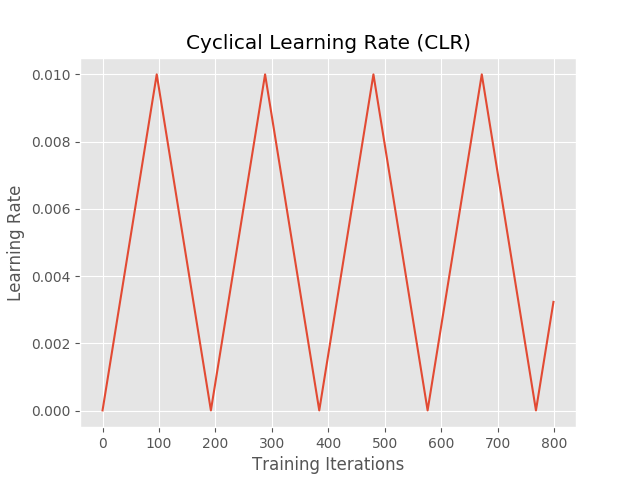
\includegraphics[scale=0.67]{images/baseline/clr_plot_triangular_6.png} 
\label{i_baseline_tr}
\caption{Andamento del metodo Triangular con step size 6}
\end{figure}

\begin{figure}[H]
\centering
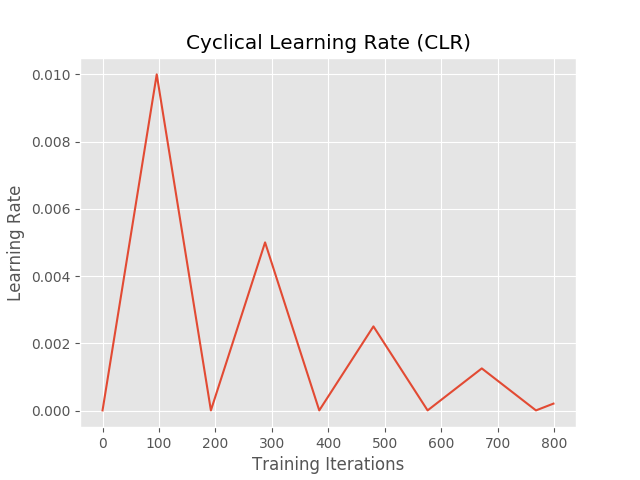
\includegraphics[scale=0.67]{images/baseline/clr_plot_triangular2_6.png} 
\label{i_baseline_tr2}
\caption{Andamento del metodo Triangular2 con step size 6}
\end{figure}
Da questa prima valutazione si è in grado di notare come il preaddestramento sia già in grado di discriminare con una buona accuratezza le diverse classi da cui è composto il dataset.
\subsection{Esperimento 1 - Finetuning Resnet-18}
La sola estrazione delle feature non è ovviamente abbastanza per ottenere delle performance soddisfacenti sul test set, si è proceduto quindi ad eseguire il finetuning dell'intera rete in modo tale da aggiornare i pesi per renderli più compatibili con il nuovo dataset.
Adesso invece di accodare un percettrone multistrato all'ultimo layer della rete viene invece applicato un average pooling seguito da un layer di dropout ed un layer completamente connesso contenente 102 neuroni.
\subsubsection{Preprocessing e Data augmentation}
Per massimizzare la generalizzazione del modello si è deciso di "aumentare" le immagini di training applicando i seguenti effetti durante la fase di training:
\begin{itemize}
\item Flip orizzontale
\item Aumento/riduzione della luminosità 
\item Rotazione in un angolo di $\pm$ 10°
\end{itemize}
Le immagini vengono poi normalizzate in accordo con la media e la varianza di \textit{Imagenet} come descritto nella sezione precedente.
\subsubsection{Scelta degli iperparametri}
L'ottimizzatore utilizzato in questo caso è Adam, questo tipo di ottimizzatore definisce un learning rate adattivo per ogni layer (verificare!!!) per questo motivo dovrebbe applicare un learning rate più basso per i layer all'inizio della rete ed uno più alto per gli ultimi layer che dovrebbero modificarsi maggiormente per adattarsi al nuovo dataset.
Per addestrare la rete e trovare il miglior learning rate vengono utilizzate le stesse tecniche descritte nella sezione precedente.


This is the central and most important section of the report. Its objective must be to show, with linearity and clarity, the steps that have led to the definition of a decision model. The description of the working hypotheses, confirmed or denied, can be found in this section together with the description of the subsequent refining processes of the models. Comparisons between different models (e.g. heuristics vs. optimal models) in terms of quality of solutions, their explainability and execution times are welcome. 

Do not attempt to describe all the code in the system, and do not include large pieces of code in this section, use pseudo-code where necessary. Complete source code should be provided separately (in Appendixes, as separated material or as a link to an on-line repo). Instead pick out and describe just the pieces of code which, for example:
\begin{itemize}
\item are especially critical to the operation of the system;
\item you feel might be of particular interest to the reader for some reason;
\item  illustrate a non-standard or innovative way of implementing an algorithm, data
structure, etc..
\end{itemize}

You should also mention any unforeseen problems you encountered when implementing the
system and how and to what extent you overcame them. Common problems are:
 difficulties involving existing software.

\section{Esperimento 0}
\subsubsection{Preprocessing e Data augmentation}
Per massimizzare la generalizzazione del modello si è deciso di "aumentare" le immagini di training applicando i seguenti effetti durante la fase di training:
\begin{itemize}
\item Flip orizzontale
\item Aumento/riduzione della luminosità 
\item Rotazione in un angolo di $\pm$ 10°
\end{itemize}
Le immagini vengono poi normalizzate per avere media nulla e varianza unitaria utilizzando la formula:
\begin{equation}
x' = \frac{x - \overline{x}}{\sigma}
\end{equation}
Dove $ \overline{x} $ e $ \sigma $ rappresentano rispettivamente la media e la varianza calcolate su \textit{Imagenet}
\section{Results and Evaluation}
The Results section is dedicated to presenting the actual results (i.e. measured and calculated quantities), not to discussing their meaning or interpretation. The results should be summarized using appropriate Tables and Figures (graphs or schematics). Every Figure and Table should have a legend that describes concisely what is contained or shown. Figure legends go below the figure, table legends above the table. Throughout the report, but especially in this section, pay attention to reporting numbers with an appropriate number of significant figures. 

\section{Discussion}
The discussion section aims at interpreting the results in light of the project's objectives. The most important goal of this section is to interpret the results so that the reader is informed of the insight or answers that the results provide. This section should also present an evaluation of the particular approach taken by the group. For example: Based on the results, how could the experimental procedure be improved? What additional, future work may be warranted? What recommendations can be drawn?


\section{Conclusions}
Conclusions should summarize the central points made in the Discussion section, reinforcing for the reader the value and implications of the work. If the results were not definitive, specific future work that may be needed can be (briefly) described. The conclusions should never contain ``surprises''. Therefore, any conclusions should be based on observations and data already discussed. It is considered extremely bad form to introduce new data in the conclusions.

\section*{References}

The references section should contain complete citations following standard form.  The references should be numbered and listed in the order they were cited in the body of the report. In the text of the report, a particular reference can be cited by using a numerical number in brackets as \cite{Lee2015} that corresponds to its number in the reference list. \LaTeX provides several styles to format the references

\bibliographystyle{IEEEtran}
\bibliography{references.bib}

\end{document}
